\section{Experimental Evaluation}\label{sec:experiments}

In this section we present our experimental results in four parts.
\begin{enumerate}
    \item In Section~\ref{sec:eval_pddl+} we compare the performance of SMTPlan against other PDDL+ planners on PDDL+ benchmarks for hybrid systems domains. We aim to show that in problems with non-linear continuous change, and a small number of happenings, SMTPlan performs very well.
    
    \item In Section~\ref{sec:eval_objects} we investigate the scalability of SMTPlan in PDDL+ domains in more detail.
    
    \item In Section~\ref{sec:eval_pddl21} we compare SMTPlan with temporal planners from the International Planning Competition (IPC) on a set of temporal planning benchmarks used in the IPC. In the experiment we explore the limitations inherent in the Satisfiability approach in terms of scalability with respect to the size of the discrete state-space.
    
    \item Finally, in Section~\ref{sec:eval_cp} we evaluate the effect of control parameters on our encoding, comparing the effectiveness of SMTPlan on two versions of the same domain, with and without control parameters.
\end{enumerate}

\subsection{PDDL+ Benchmarks}\label{sec:eval_pddl+}

We use our encoding to solve PDDL+ planning problems with a parallel iterative deepening technique, widely used in SAT-based planning approaches~\cite{nab02,rin06}. The top-level algorithm encodes and solves $n$ SMT encodings simultaneously, solving the planning problem for horizon lengths $1,2,3,4,...,n$. In this case, horizon length corresponds to number of happenings. If a formula is found satisfiable, then a plan has been found and the planner terminates. If a formula is found unsatisfiable, then an encoding is made for the next shortest horizon length, so that there are always $n$ SMT instances being solved. The SMT solver we use is z3~\cite{dem08}.

We compare our approach (called SMTPlan) against existing PDDL+ planner UPMurphi~\cite{upmurphi}, and with dReach~\cite{bryce}, using the SMT solver dReal~\cite{gao12}, on domains both with and without events\footnote{We considered domains without events as we wanted to show the comparison with dReach which does not handle domains including events}. We use the \textit{generator} and \textit{car} domains~\cite{bogomolov14}. The experiments were run using 8GB of RAM and a 30 minute timeout. All test domains and problems are available at: \textit{kcl-planning.github.io/SMTPlan}.

The generator domain is a PDDL+ benchmark problem that revolves around refueling a diesel-powered generator, which has to run for a given duration without overflowing or running dry. To test scalability the number of tanks is increased while decreasing the initial fuel level.

We consider four versions of this domain: linear, simplified-nonlinear (the same used in ~\cite{bryce}), nonlinear with events, and the Torricelli nonlinear~\cite{howey2003val}. Note that the latter version uses the Torricelli's Law (which is too complex for dReach), and hence the fuel level in a refueling tank ($V_{fuel}$) is calculated by:

\begingroup\makeatletter\def\f@size{10}\check@mathfonts
\begin{equation}
	V_{fuel} = (-kt_r+\sqrt[]{V_{init}})^2 \qquad t_r \in \left[0, \frac{\sqrt[]{V_{init}}}{k}\right] 
\end{equation}
\label{vol_eq}
\endgroup

where $V_{init}$ is the initial volume of fuel in the tank, $k$ is the fuel flow constant (which depends on gravity, size of the drain hole, and the cross-section of the tank), and $t_r$ is the time of refueling (bounded by the fuel level and the flow constant). An example of plan found by SMTPlan for the Torricelli nonlinear generator (Fuel level 960, Generator capacity 990) is shown in Figure~\ref{fig:generatorplan}:

\begin{figure}[htb!]
\centering
\small
\begin{BVerbatim}
0.0: generate     [1000.0]
959.0: refuel_tank1 [10.0]
959.0: refuel_tank2 [10.0]
\end{BVerbatim}
\caption{Plan for a problem in the Toricelli Generator domain.}
\label{fig:generatorplan}
\end{figure}

The car domain is another PDDL+ benchmark~\cite{pddl+} where a vehicle has to cover a given distance and have a zero velocity at the end, and the actions available are accelerate and decelerate that increments or decrements by 1 the current velocity, respectively.
To test scalability, the bound on maximum acceleration/deceleration is increased.

Our results for solvable instances are reported in Table~\ref{tab:solvable}. On both linear and nonlinear domains, SMTPlan outperforms all other planners in time to solve and in number of instances solved. In all domains, SMTPlan scales very well. For these domains, the number of happenings required is small, thus the minimal SMT encoding required to solve the problem is also small. The iterative deepening algorithm is able to reach a satisfiable encoding, and produce a plan very quickly. The offline computation with SymPy is required only once per domain, and in all cases required 0.3 seconds or less.

dReach also performs iterative deepening, but performs more poorly. This is due to the semantics of dReach; in the dReach domain and problem description, each mode of continuous change must be explicitly defined, and the number of modes increases exponentially with the number of processes and durative actions (eg. the files for 1, 2, 3 and 4 tanks problems are respectively 91, 328, 1350, 5762 lines long). Furthermore, the bound is not on the number of happenings, but on the number of mode changes, which does not allow for parallel execution of actions.

Moreover, dReach does not perform integration and differentiation outside of the solver, during encoding. Instead it relies upon the more expressive logic of the internal SMT solver, dReal, at the cost of extra computation time. In addition, they are unable to use SMT solvers other than dReal.

We also compare our encoding directly against dReach as reported in prior work~\cite{bryce}: reporting times to solve only the encoding of a minimal step plan for each instance (table~\ref{tab:finalstep}). These are not the times required to solve a PDDL+ instance, but a direct comparison of encodings on satisfiable problems. We find the encodings exhibit similar performance in the car domain. However, we find the SMTPlan encoding scales far better on the generator problem, as discussed above. Moreover, the SMTPlan encoding does not require the advanced features of dReal, and can be solved more quickly using z3.

Our results for unsolvable instances are shown in table~\ref{tab:unsolvable}. SMTPlan and dReach can only prove unsolvability up to an upper bound on the number of happenings. Here we prove plan non-existence for domains which have a tight deadline, and where each ground action can only be applied a finite number of times. We also include SpaceEx that can be used to prove plan-non existence for the generator linear domain~\cite{bogomolov14}. We observe that both totally ordered planning approaches perform well proving unsolvability in the car domain. There are few choices of symbolic plan in this domain, leaving only the timing of the happenings and numeric constraints to be solved. Both SMTPlan and dReach solve these constraints very quickly. However, for PDDL+ problems in general, without deadlines and with repeatable actions, proving unsolvability is difficult through totally ordered planning with iterative deepening.

\begin{table*}[ht]
\centering
\def\arraystretch{1.2}
\begin{tabular}{|p{6em}|l|cccccccc|}
\hline
Domain         & Tool      & 1    & 2    & 3    & 4    & 5    & 6    & 7    & 8     \\
\hline
\multirow{3}{*}{\parbox{6em}{Generator linear}}
               & SMTPlan  & 0.02  & 0.03 & 0.02   & 0.01  & 0.02 & 0.02 & 0.02 & 0.02  \\
               & dReach    & 2.87  & -    & -      & -     & -    & -    & -    & -     \\
               & UPMurphi  & 0.2  & 18.2 & 402.34  & -     & -    & -    & -    & -     \\ % results from Bogolomov
\hline \hline
\multirow{3}{*}{\parbox{6em}{Generator nonlinear}}
               & SMTPlan  & 0.02  & 0.02 & 0.02   & 0.02  & 0.02  & 0.02  & 0.02    & 0.02   \\
               & dReach    & 5.16  & -    & -      & -     & -     & -     & -       & -      \\
               & UPMurphi  & 63.16 & -    & -      & -     & -     & -     & -       & -      \\
\hline \hline
\multirow{3}{*}{\parbox{6em}{Generator nonlin. events}}
               & SMTPlan  & 0.04 & 0.04 & 0.04 & 0.04  & 0.04 & 0.04 & 0.05 & 0.05  \\
               & dReach    & x    & x    & x    & x     & x    & x    & x    & x     \\
               & UPMurphi  & 658.18 & -    & -    & -     & -    & -    & -    & -     \\
\hline \hline
\multirow{3}{*}{\parbox{6em}{Generator Torricelli}}
               & SMTPlan  & 0.03  & 0.03 & 0.15 & 0.92  & 0.04 & 0.05 & 0.09 & 0.50  \\
               & dReach    & x     & x    & x    & x     & x    & x    & x    & x     \\
               & UPMurphi  & 63.16 & -    & -    & -     & -    & -    & -    & -     \\
\hline \hline
\multirow{3}{*}{\parbox{6em}{Car}}
               & SMTPlan  & 0.02  & 0.02  & 0.02 & 0.02  & 0.02 & 0.02 & 0.01 & 0.02  \\
               & dReach    & 1.30  & 1.41  & 1.48 & 1.53  & 1.47 & 1.54 & 1.40 & 1.53  \\
               & UPMurphi  & 28.44 & 386.5 & -    & -     & -    & -    & -    & -     \\ % results from Bogolomov
\hline
\end{tabular}
\caption{Results in seconds for solvable instances. Instance numbers correspond to number of tanks (generator) and number of acceleration steps (car). Abbrev.: ’-’: tool still running after 30 minutes, '.': tool ran out or memory, ’x’: tool cannot handle the problem.}
\label{tab:solvable}
\end{table*}

\begin{table*}[ht]
\centering
\def\arraystretch{1.2}
\begin{tabular}{|l|l|cccccccc|}
\hline
Domain         & Tool      & 1    & 2      & 3     & 4    & 5      & 6    & 7    & 8     \\
\hline
\multirow{3}{*}{\parbox{6em}{Generator linear}}
               & SMTPlan & 0.01 & 0.02   & 0.16  & 2.84 & 390.86  & -    & -    & -     \\
               & dReach    & 2.57 & 189.94 & -     & -    & -      & -    & -    & -     \\
               & UPMurphi  & 0.90 & 29.42  & -     & -    & -      & -    & -    & -     \\ % results from Bogolomov
\hline \hline
\multirow{3}{*}{\parbox{6em}{Generator nonlinear}}
               & SMTPlan  & 0.01 & 1.95   & 33.48 & -    & -      & -    & -    & -     \\
               & dReach    & 2.43 & 212.43 & -     & -    & -      & -    & -    & -     \\
               & UPMurphi  & -    & -      & -     & -    & -      & -    & -    & -     \\
\hline \hline
\multirow{3}{*}{\parbox{6em}{Generator nonlin. events}}
               & SMTPlan  & 0.02   & 18.58   & 21.83 & -    & -      & -    & -    & -     \\
               & dReach    & x      & x       & x     & x    & x      & x    & x    & x     \\
               & UPMurphi  & -      & -       & -     & -    & -      & -    & -    & -     \\
\hline \hline
\multirow{3}{*}{\parbox{6em}{Generator Toricelli}}
               & SMTPlan  & 0.03  & 2.06   & 19.57 & -    & -      & -    & -    & -     \\
               & dReach    & x     & x      & x     & x    & x      & x    & x    & x     \\
               & UPMurphi  & -     & -      & -     & -    & -      & -    & -    & -     \\
\hline \hline
\multirow{3}{*}{\parbox{6em}{Car}}
               & SMTPlan  & 0.68  & 0.02   & 0.00  & 0.00 & 0.00   & 0.00 & 0.00 & 0.01  \\
               & dReach    & 0.67  & 0.50   & 0.62  & 0.45 & 0.58   & 0.57 & 0.49 & 0.65  \\
               & UPMurphi  & 36.01 & 445.23 & -     & -    & -      & -    & -    & -     \\ % results from Bogolomov
\hline
\end{tabular}
\caption{Results in seconds for unsolvable instances. Instance numbers correspond to number of tanks (generator) and number of acceleration steps (car). Abbrev.: ’-’: tool still running after 30 minutes, ’x’: tool cannot handle the problem.}
\label{tab:unsolvable}
\end{table*}

\begin{table*}[ht]
\centering
\def\arraystretch{1.1}
\begin{tabular}{|l|l|cccccccc|}
\hline
Domain         & Tool      & 1     & 2    & 3    & 4    & 5    & 6    & 7     & 8     \\
\hline

\multirow{2}{*}{\parbox{6em}{Generator linear}}
               & SMTPlan  & 0.00  & 0.01  & 0.01   & 0.01   & 0.01 & 0.02 & 0.02  & 0.02  \\
               & dReach    & 2.73  & 13.47 & 104.61 & 695.70 & -    & -    & -     & -     \\
\hline \hline
\multirow{2}{*}{\parbox{6em}{Generator nonlinear}}
               & SMTPlan  & 0.01  & 0.01    & 0.01 & 0.01   & 0.01 & 0.01 & 0.01  & 0.01 \\
               & dReach    & 10.42 & 1685.35 & -    & -      & -    & -    & -     & -    \\
\hline \hline
\multirow{2}{*}{\parbox{6em}{Car}}
               & SMTPlan  & 0.00  & 0.00 & 0.00 & 0.00 & 0.00 & 0.00 & 0.00 & 0.00  \\
               & dReach    & 0.77  & 0.76 & 0.76 & 0.76 & 0.76 & 0.76 & 0.77 & 0.76  \\
\hline
\end{tabular}
\caption{Results in seconds for minimal step encoding required to solve each instance.}
\label{tab:finalstep}
\end{table*}

\subsection{Free Fall and Generator}\label{sec:eval_objects}

Furthermore we designed two new sets of experiments. The first experiment evaluates the effects of having multiple objects in the domain file. 

\smallskip

For this mean we have expanded the \textit{Free Fall} problem and considered problem instances where we have more than one ball in our problem file.  

We considered two scenarios for these problem instances. In both scenario we increase the number of balls in the problem file. We create cases that include 25,50 ,100 and 200 balls. In the first scenario we try to find a plan for a set of problem instances while the goal state is to catch just the first ball. As we can see in Figure~\ref{fig:Picture1}, as we increase the number of balls in the problem file, the time needed to solve the problem increases linearly. However, by increasing the number of balls, the search space grows exponentially. SMTPlan focuses on variables related to the objects from the problem file that are involved in the goal state and tries to find the assignments for them. In other word, it also propagates the search branches regarding the variables that are representing other objects that are not in the goal state.

%This means SMTPlan notices that the SMT variables related to the object that is in the goal state is the critical on and tries to solve them and propagate the other variables of the other objects. 

In the second scenario we continued the experiments by changing the goal state to catch all the balls in the problem file (we considered all the balls have the same initial height and we want to catch all of them at a certain height). Figure~\ref{fig:Picture1} indicates the results of catching all the balls in the cases we used before. As it is shown the trend of the total time needed to solve the problem is linear. All the plans obtained from SMTPlan suggest to release all the balls together and also catch all of them at the same time point. This is resulted from the fact that SMTPlan tries to solve the problem with minimum number of happenings. Similar to the previous case, the search space grows exponentially, however this growth affects our solving time linearly as the SMTPlan tries to solve the problem with minimum number of happenings \footnote{As it is mentioned in Section~\ref{sssec:SMTPlan_Archi}, SMTPlan starts to find a plan with an initial number of happening which can be defined for it (otherwise it starts with two happening. If it can not find a plan it increases the number of happenings and this increase can be by one or a step size that can be defined for the planner. If we run the SMTPlan with the initial number of happenings of two and define that step size as one, the planner finds a planner with the minimum number of happenings, if the problem is solvable.}.  

\iffalse
\begin{figure}[tbp!]
\centering
\begin{subfigure}[b]{0.48\textwidth}
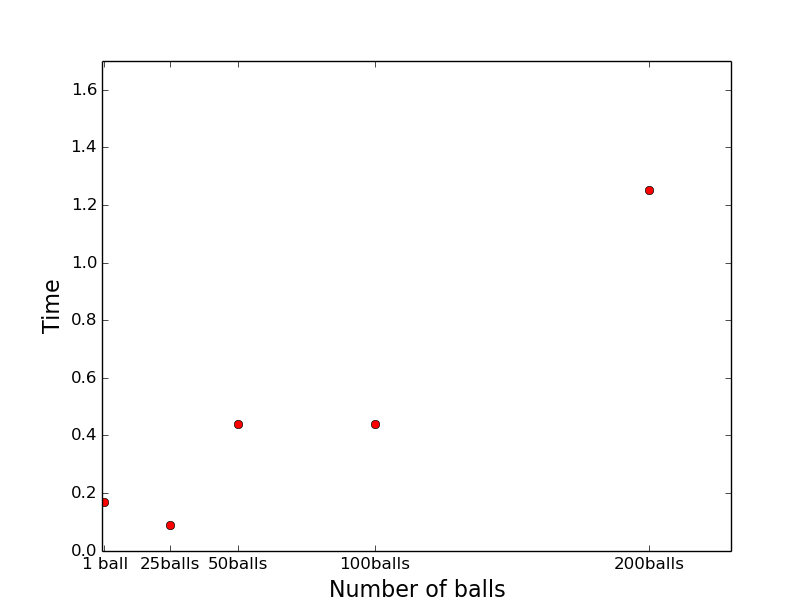
\includegraphics[width=\textwidth]{diagrams/Ball1.png}
\caption{Catch one ball}
\label{fig:Picture1}
\end{subfigure}
\hfill
\begin{subfigure}[b]{0.48\textwidth}
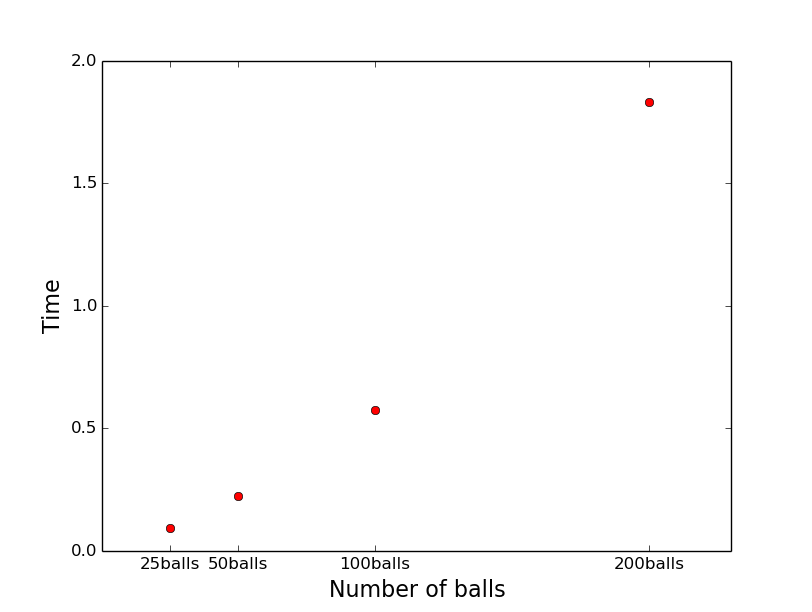
\includegraphics[width=\textwidth]{diagrams/Ball2.png}
\caption{Catch all the balls}
\label{fig:Picture2}
\end{subfigure}
\caption{(a):The Free Fall example with 1,25,50,100 and 200 balls. The goal is to catch the first bal.(b):The Free Fall example with 25,50,100 and 200 balls. The goal is to catch all the ball that have the same initial and goal state.}
\end{figure}
\fi

\begin{figure}[!ht]
\centering
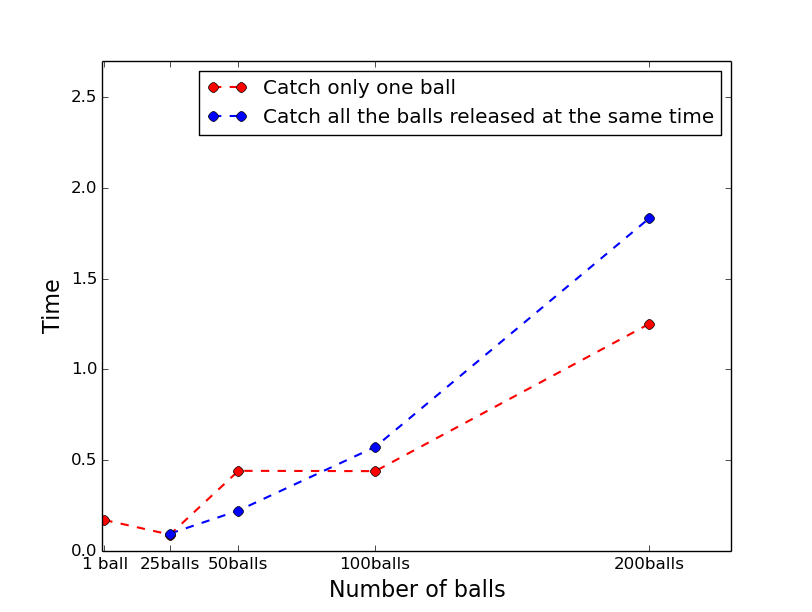
\includegraphics[width=0.80\textwidth]{diagrams/Balls.png}
\caption{The bar chart compares the time taken for SMTPlan to solve the free fall problem. The blue bars indicate the scenarios that we have 1,25,50,100 and 200 balls and the aim of the problem is to just catch the first call. The green bars represents the scenarios that we have 25,50,100 and 200 balls and the goal is to catch all of them.}
\label{fig:Picture1}
\end{figure}

We also tested the performance of the SMTPlan when we have domains with actions that have longer time horizon. For this mean we used two different generator domains and generated a number of problems when the capacity of the generator and the running time of it increase gradually. In the initial problem the running time of the generator is $\num{1.000}$ seconds, however we tested problems where the generator has running times of$\num{2.000}$, $\num{3.000}$, $\num{5.000}$ and $\num{20.000}$ time units. As we wanted to test the effects of the time horizon on the planner, we also changed the initial amount of the fuel in the tank, so the number of times that we need to apply the re-fuelling action remains the same. In other words, just the length of the re-fuelling process has been extended. As you can see in Figures~\ref{fig:Picture4} and ~\ref{fig:Picture3}, we have done the test both using SMTPlan and DiNo. SMTPlan has shown that the time to find a plan is not related to the time horizon of the actions (as we increase the time horizon the time needed to to find the plan for SMTPln remains the same). However, as we increase the time horizon, DiNo needs longer time to solve the problem. This can be explained by the fact that, DiNo needs to discretised the time and as we have a longer time horizon the search space grows and the planner needs more time to find the plan. On the other hand for the SMTPlan, since the number of the happenings are the same, increasing the time horizon won't change anything for the SMTPlan and for this reason it is able to find the plan in the same time.  

\begin{figure}[tbp!]
\centering
\begin{subfigure}[b]{0.49\textwidth}
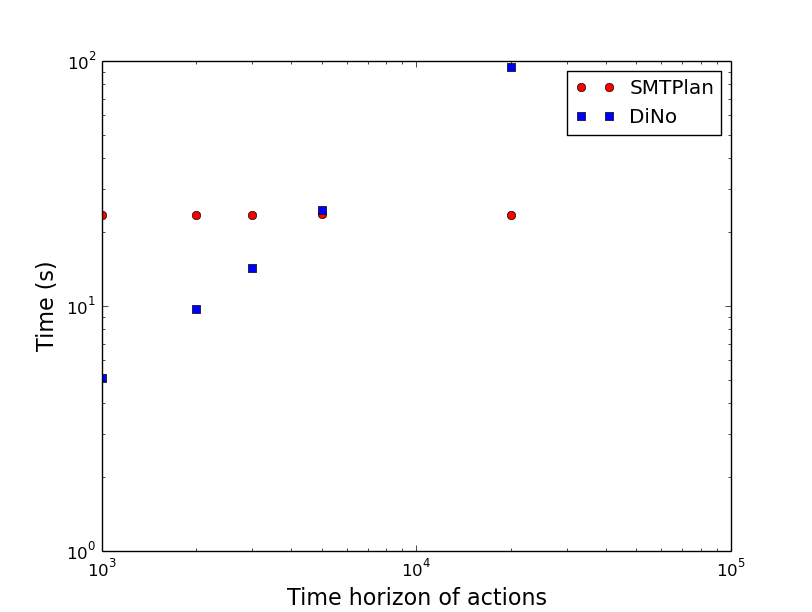
\includegraphics[width=0.80\textwidth]{diagrams/Generator_event.png}
\caption{}
\label{fig:Picture4}
\end{subfigure}
\hfill
\begin{subfigure}[b]{0.48\textwidth}
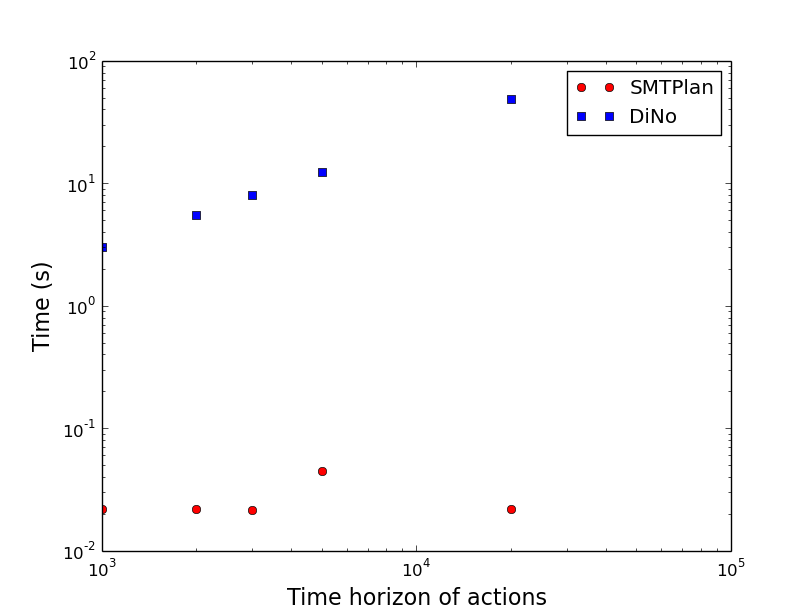
\includegraphics[width=0.80\textwidth]{diagrams/Generator_linear.png}
\caption{}
\label{fig:Picture3}
\end{subfigure}
\caption{Generator domain with (a)events/ (b)linear continuous changes with different time horizons}
\end{figure}



\iffalse
\begin{figure}[!ht]
\centering
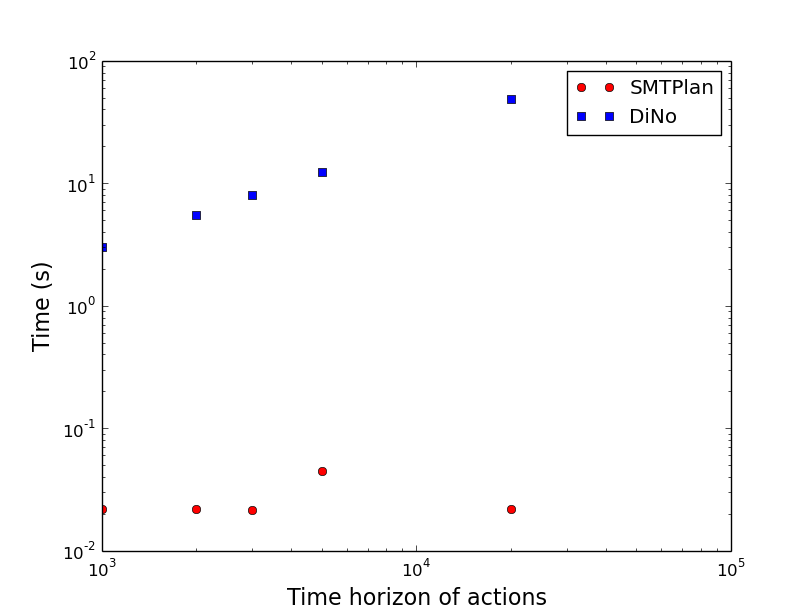
\includegraphics[width=0.80\textwidth]{diagrams/Generator_linear.png}
\caption{Generator domain with linear continuous changes with different time horizons}
\label{fig:Picture4}
\end{figure}
\fi
\subsection{Temporal Domains}\label{sec:eval_pddl21}

For the sake of completeness, we also tested the SMTPlan on the temporal domains that are used in the temporal track at ICAPS 2018. The results are shown in Table~\ref{tab:ipc result}. We compared the SMTPlan with the other planners participated in this track. These planners are CP4TP  ~\cite{cp4tp}, TFLAP  ~\cite{tflap}, TemPorAl  ~\cite{temporal}, PopCorn  ~\cite{popcorn} and OPTIC  ~\cite{OPTIC}. 

The time given to each planner was 30 minutes and 8GB of memory. In total 10 domains have been chosen and for each domain 10 problem instances have been selected. Each number in the table indicates the number of problem instances that each planner has managed to solve. At each raw, for each domain, the maximum number of problems that is solved is shown in bold. 



\begin{table}[thb]
\centering
\begin{tabular}{|l|l|l|l|l|l|l|l|}

\hline
                   &     & \multicolumn{6}{c|}{Planners}                                                 \\ \hline
Domain             & N   & SMTPlan     & CP4TP       & TFLAP       & TemPorAl    & PopCorn & OPTIC       \\ \hline
Airport            & 10  & 1           & 9           & 9           & \textbf{10} & 3       & 3           \\ \hline
Cushing            & 10  & \textbf{10} & \textbf{10} & 3           & 0           & 1       & \textbf{10} \\ \hline
Floortile          & 10  & 0           & 2           & 3           & \textbf{10} & 0       & 0           \\ \hline
Map Analyser       & 10  &             & \textbf{10} & 8           & \textbf{10} & 0       & 0           \\ \hline
Parking            & 10  & 0           & \textbf{10} & \textbf{10} & \textbf{10} & 4       & 8           \\ \hline
Quantum            & 10  & 1           & \textbf{10} & 8           & \textbf{10} & 5       & 8           \\ \hline
Road Traffic       & 10  & 0           & 7           & 0           & \textbf{10} & 0       & 0           \\ \hline
Sokoban            & 10  & 0           & \textbf{6}  & 4           & \textbf{6}  & 1       & 1           \\ \hline
Trucks-time-strips & 10  & 0           & \textbf{10} & \textbf{10} & \textbf{10} & 9       & \textbf{10} \\ \hline
Total              & 100 & 12          & 74          & 55          & \textbf{76} & 23      & 40          \\ \hline
\end{tabular}
\caption{Results in the number of problems that each planner could solve for the domains from ICAPS 2018 temporal tracks}
\label{tab:ipc result}
\end{table}

\subsection{Domains with Control Parameters}\label{sec:eval_cp}

In this section we have designed a set of experiments to show how introducing control parameters affects the performance of SMTPlan. We used the \textit{cashpoint} domain for this experiments. We did the same experiments using two different types of the same domain; one domain including control parameter variables and the other one without. For both domains we considered a set of problem instances that get more difficult gradually. We increased the difficulty of the problems in two ways: first, by adding new objects in the problem file; and second, by considering scenarios in which we have more actions in the domain file and in order to reach the goal we need to apply these new actions. 


First we create a set of problem instances. The goal of all these problem files is to have a specific amount of money, which is indicated by the variable  $(inpocket \ \ pounds)$ in the goal state. We have started from $( = (inpocket \ \ pounds) 10) $ and with increments of 10 unites and it reaches to  $( = (inpocket \ \ pounds) 100) $. Moreover, in order to make more difficult problems, the number of objects in each problem file is increased. We first start the problems with just one bank, then increase them to 6 banks. For all the experiments in this section, we have used these set of benchmarks. 

We also added more propositions to the goal state, which leads to plans with more actions. The goal of the first scenario is just to withdraw money. Then, we gradually make increase the difficulty of the domain by adding new actions. The next considered scenario is a domain in which we need to go from home to bank and then withdraw money. For the third case we considered that we need to go to the pub at the end and in the last scenario we need to go the supermarket and get some snacks as well. 

%In the first scenario, the goal was to have specific amount of money and for this we just need to apply one type of action $(withdraw\_money)$. Then we run the same domain for several problems and increased the objects in each problem instance (we increased the number of banks in each problem and also designed the problem in the way that in order to have enough $(inpocket \ \ pounds)$ we need to withdraw from all the banks). Then we made the problem harder in the second scenario by adding a new goal that we are at home and we want to have specific amount of money. In order to achieve the goal we need to apply two actions $(go\_to)$ and $(withdraw\_money)$. Then we run them with the same set of problems that was getting hard gradually. Then for the third scenario, we changed the problem file and added a new proposition to the goal that we need to be at pub at the end. Then at the 4th, 5th and 6th scenarios we add the facts that we need to buy snacks, drinks and shoes from supermarket gradually and run them with the same set of problems. 



The result for these experiments are shown in ~\ref{fig:CP_results}. The $y$ axis shows the results of the experiments for domains without control parameters and the $x$ axis is for domains with control parameters. The time given to the solver for these set of experiments was 3600 seconds. As we can see on the graph, the time to solve the problems without control parameters are much longer compare to the domains with control parameters. 

\begin{figure}[!ht]
\centering
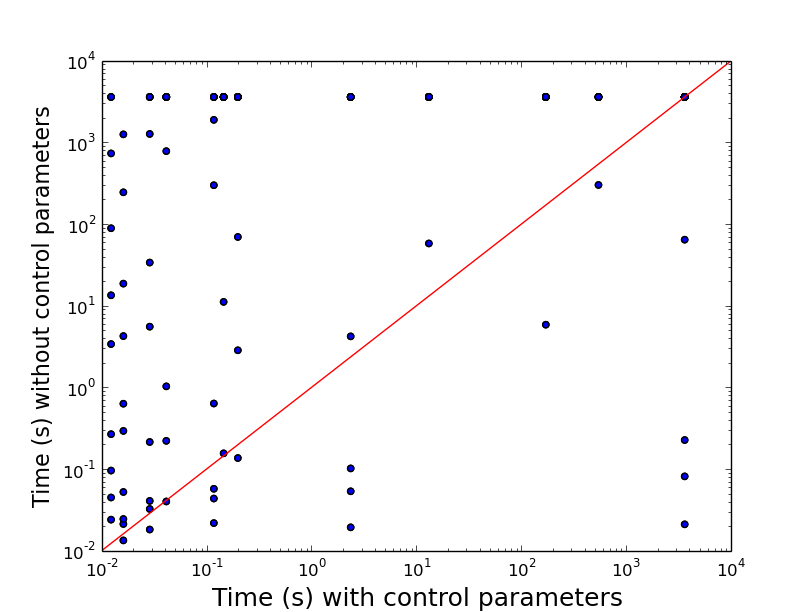
\includegraphics[width=0.60\textwidth]{diagrams/CP_results.png}
\caption{The results of running SMTPlan for cashpoint example. The experiment compares the time taken to solve the cashpoint problems using two domains: (a) the domain without having control parameter variables (b) same domain with durative action which have control parameters}
\label{fig:CP_results}
\end{figure}


Moreover, the number of problems that domain's with control parameters can solve is compared in Table ~\ref{tab:table_results_cp}.

\begin{table}[!ht]
\centering
\begin{tabular}{|c|c|c|c|}
\hline
\multirow{2}{*}{Domain} & \multirow{2}{*}{\begin{tabular}[c]{@{}c@{}}Total number \\ \\ of problems\end{tabular}} & \multicolumn{2}{c|}{Planner}                                                                                                                             \\ \cline{3-4} 
                        &                                                                                         & \begin{tabular}[c]{@{}c@{}}SMTPlan\\ with control parameters\end{tabular} & \begin{tabular}[c]{@{}c@{}}SMTPlan\\ without control parameters\end{tabular} \\ \hline
Domain0                 & 60                                                                                      & 50                                                                        & 39                                                                           \\ \hline
Domain1                 & 40                                                                                      & 30                                                                        & 7                                                                            \\ \hline
Domain2                 & 30                                                                                      & 20                                                                        & 4                                                                            \\ \hline
Domain3                 & 20                                                                                      & 10                                                                        & 1                                                                            \\ \hline
\end{tabular}

\caption{Comparison of number of domains that can be solved by SMTPlan that has control parameters and without control parameters}
\label{tab:table_results_cp}


\end{table}